\documentclass[a4paper,10pt]{scrartcl}

% Hier die Nummer des Blatts und Autoren angeben.
\newcommand{\blatt}{9}
\newcommand{\autor}{Florian B\"ohm, Christopher Gawehn, Ulrike Geries, Jim Martens}

\usepackage{hci}
\usepackage[utf8]{inputenc}
\usepackage{float}
\usepackage[official]{eurosym}
\usepackage[parfill]{parskip}

\begin{document}
% Seitenkopf mit Informationen
\kopf
\renewcommand{\figurename}{Figure}

\aufgabe{1}

Dieser Bericht ist nach den Teilaufgaben strukturiert und weißt keinen durchgehenden Erzählstrang auf.
	\begin{enumerate}
		\item 
		Die App läuft auf einem touchfähigen Smartphone ohne Tasten. Dabei geschieht die Ausgabe sowohl über das Display als auch in Form von Strahlung oder WLAN, die eine Aktion beim Fernseher durchführt. Die App muss sowohl bei Helligkeit als auch bei Dunkelheit funktionieren. Ebenso darf sie für das Ausführen kein Internet benötigen.
		\item 
		Die App wird maximal von Besitzern eines touchfähigen Smartphones verwendet werden. Eine weitere Einschränkung ergibt sich aus der Umsetzung der Interaktion mit dem Fernseher. Wenn die Kommunikation über ein Netzwerk verläuft (WLAN), dann muss es ein moderner Fernseher mit Internetbefähigung sein. Läuft die Kommunikation traditionell über die Strahlung wie auch bei einer Fernbedienung, dann kann jeder Fernseher verwendet werden.
		
		Von den übrigbleibenden Personen kommen wiederum nur jene in Betracht, denen die Bedienung mit der Fernbedienung zu kompliziert ist (das Verändern der Lautstärke selber oder das Verändern des Programms bzw. Senders ist ja nicht sehr kompliziert oder komplex).
		
		Mit der App kann man die Lautstärke verändern und einen Sender aus einer Liste an Sendern auswählen. Die interessanten Sender (öffentliche und bekannte private Sender) sind oben angeordnet, sodass diese schnell ausgewählt werden können. Die weniger interessanten Sender (Werbesender und Nischensender) sind weiter unten angeordnet, sodass man keine unnötige Zeit verschwendet, um zu interessanten Sendern zu kommen. Ebenfalls verändert sich die Sortierung im Laufe der Zeit. Je häufiger ein Sender genutzt wird, desto weiter nach oben in der Liste wandert der Sender. Dadurch wird die Nutzungszeit immer weiter reduziert und damit optimiert.

		Außerdem entwickelt sich somit jede Installation der App nach einer Zeit zu einer individuell angepassten Version.
		
		Die App wird meist im Wohnzimmer verwendet werden, da dies häufig der Ort des Fernsehers ist. Da der Nutzer schnell die Lautstärke ändern und den Sender wechseln möchte, müssen diese Funktionen schnell und ohne Umwege erreichbar sein.
		\item
		Eine Fokusgruppe konnten wir terminlich nicht durchführen, da zu keinem Zeitpunkt alle Zeit hatten. Wir haben uns aber per Mail über die grundlegenden Anfordernisse einer solchen App verständigt. Auf dessen Basis wurden die nachfolgenden HTAs erstellt.
		\item HTA für Lautstärke ändern: \\
\begin{tikzpicture}[
	goal/.style={rectangle,draw,fill=yellow!40,align=left},
	plan/.style={align=left},
	level 1/.style={sibling distance=7.7em},
	nextLevel/.style={level distance=40ex},
  	nextLevel2/.style={level distance=30ex},
  	nextLevel3/.style={level distance=18ex}]
	
	\coordinate
	  child[grow=up] {node[goal,anchor=south] (start) {0. Lautstärke ändern}}
	  child[grow=down,level distance=0ex]
      [edge from parent fork down]
      % sub goals
      child {node[goal] (one) {1. Smartphone \\ einschalten}}
      child {node[goal]{2. App aufrufen}}
      child {node[goal] (three) {3. Lautstärke- \\ regler anpassen}};

	\node[plan] [below right=0.4 and -1.5 of start] {\underline{Plan 0:} \\
	  	DO 1.-3.
	  };
\end{tikzpicture}
		\newpage
		HTA für Programmauswahl: \\
		
\begin{tikzpicture}[
	goal/.style={rectangle,draw,fill=yellow!40,align=left},
	plan/.style={align=left},
	level 1/.style={sibling distance=7.7em},
	nextLevel/.style={level distance=40ex},
  	nextLevel2/.style={level distance=30ex},
  	nextLevel3/.style={level distance=18ex}]
	
	\coordinate
	  	child[grow=up] {node[goal,anchor=south] (start) {0. Programm ändern}}
	  	child[grow=down,level distance=0ex]
      	[edge from parent fork down]
      	% sub goals
      	child {node[goal] (one) {1. Smartphone \\ einschalten}}
      	child {node[goal]{2. App aufrufen}}
      	child {node[goal] (three) {3. Sender \\ auswählen}
			child[nextLevel2] {node[goal] {3.1. Auf \\ Sender \\ klicken}}
			child[nextLevel2] {node[goal] {3.2. Neuen Sender \\ auswählen aus \\ Liste}}
      	};

	\node[plan] [below right=0.4 and -1.5 of start] {\underline{Plan 0:} \\
	  	DO 1.-3.
	  };
	  \node[plan] [below left=0.4 and -1.0 of three] {\underline{Plan 3:} \\
     	DO 3.1-3.2};
\end{tikzpicture}
		\newpage
		\item Insgesamt sind nur zwei Skizzen entstanden, da es auch nicht all zu viele Variationsmöglichkeiten auf Basis der Schlüsselpfadszenarien gab.
		Designskizzen: \\
		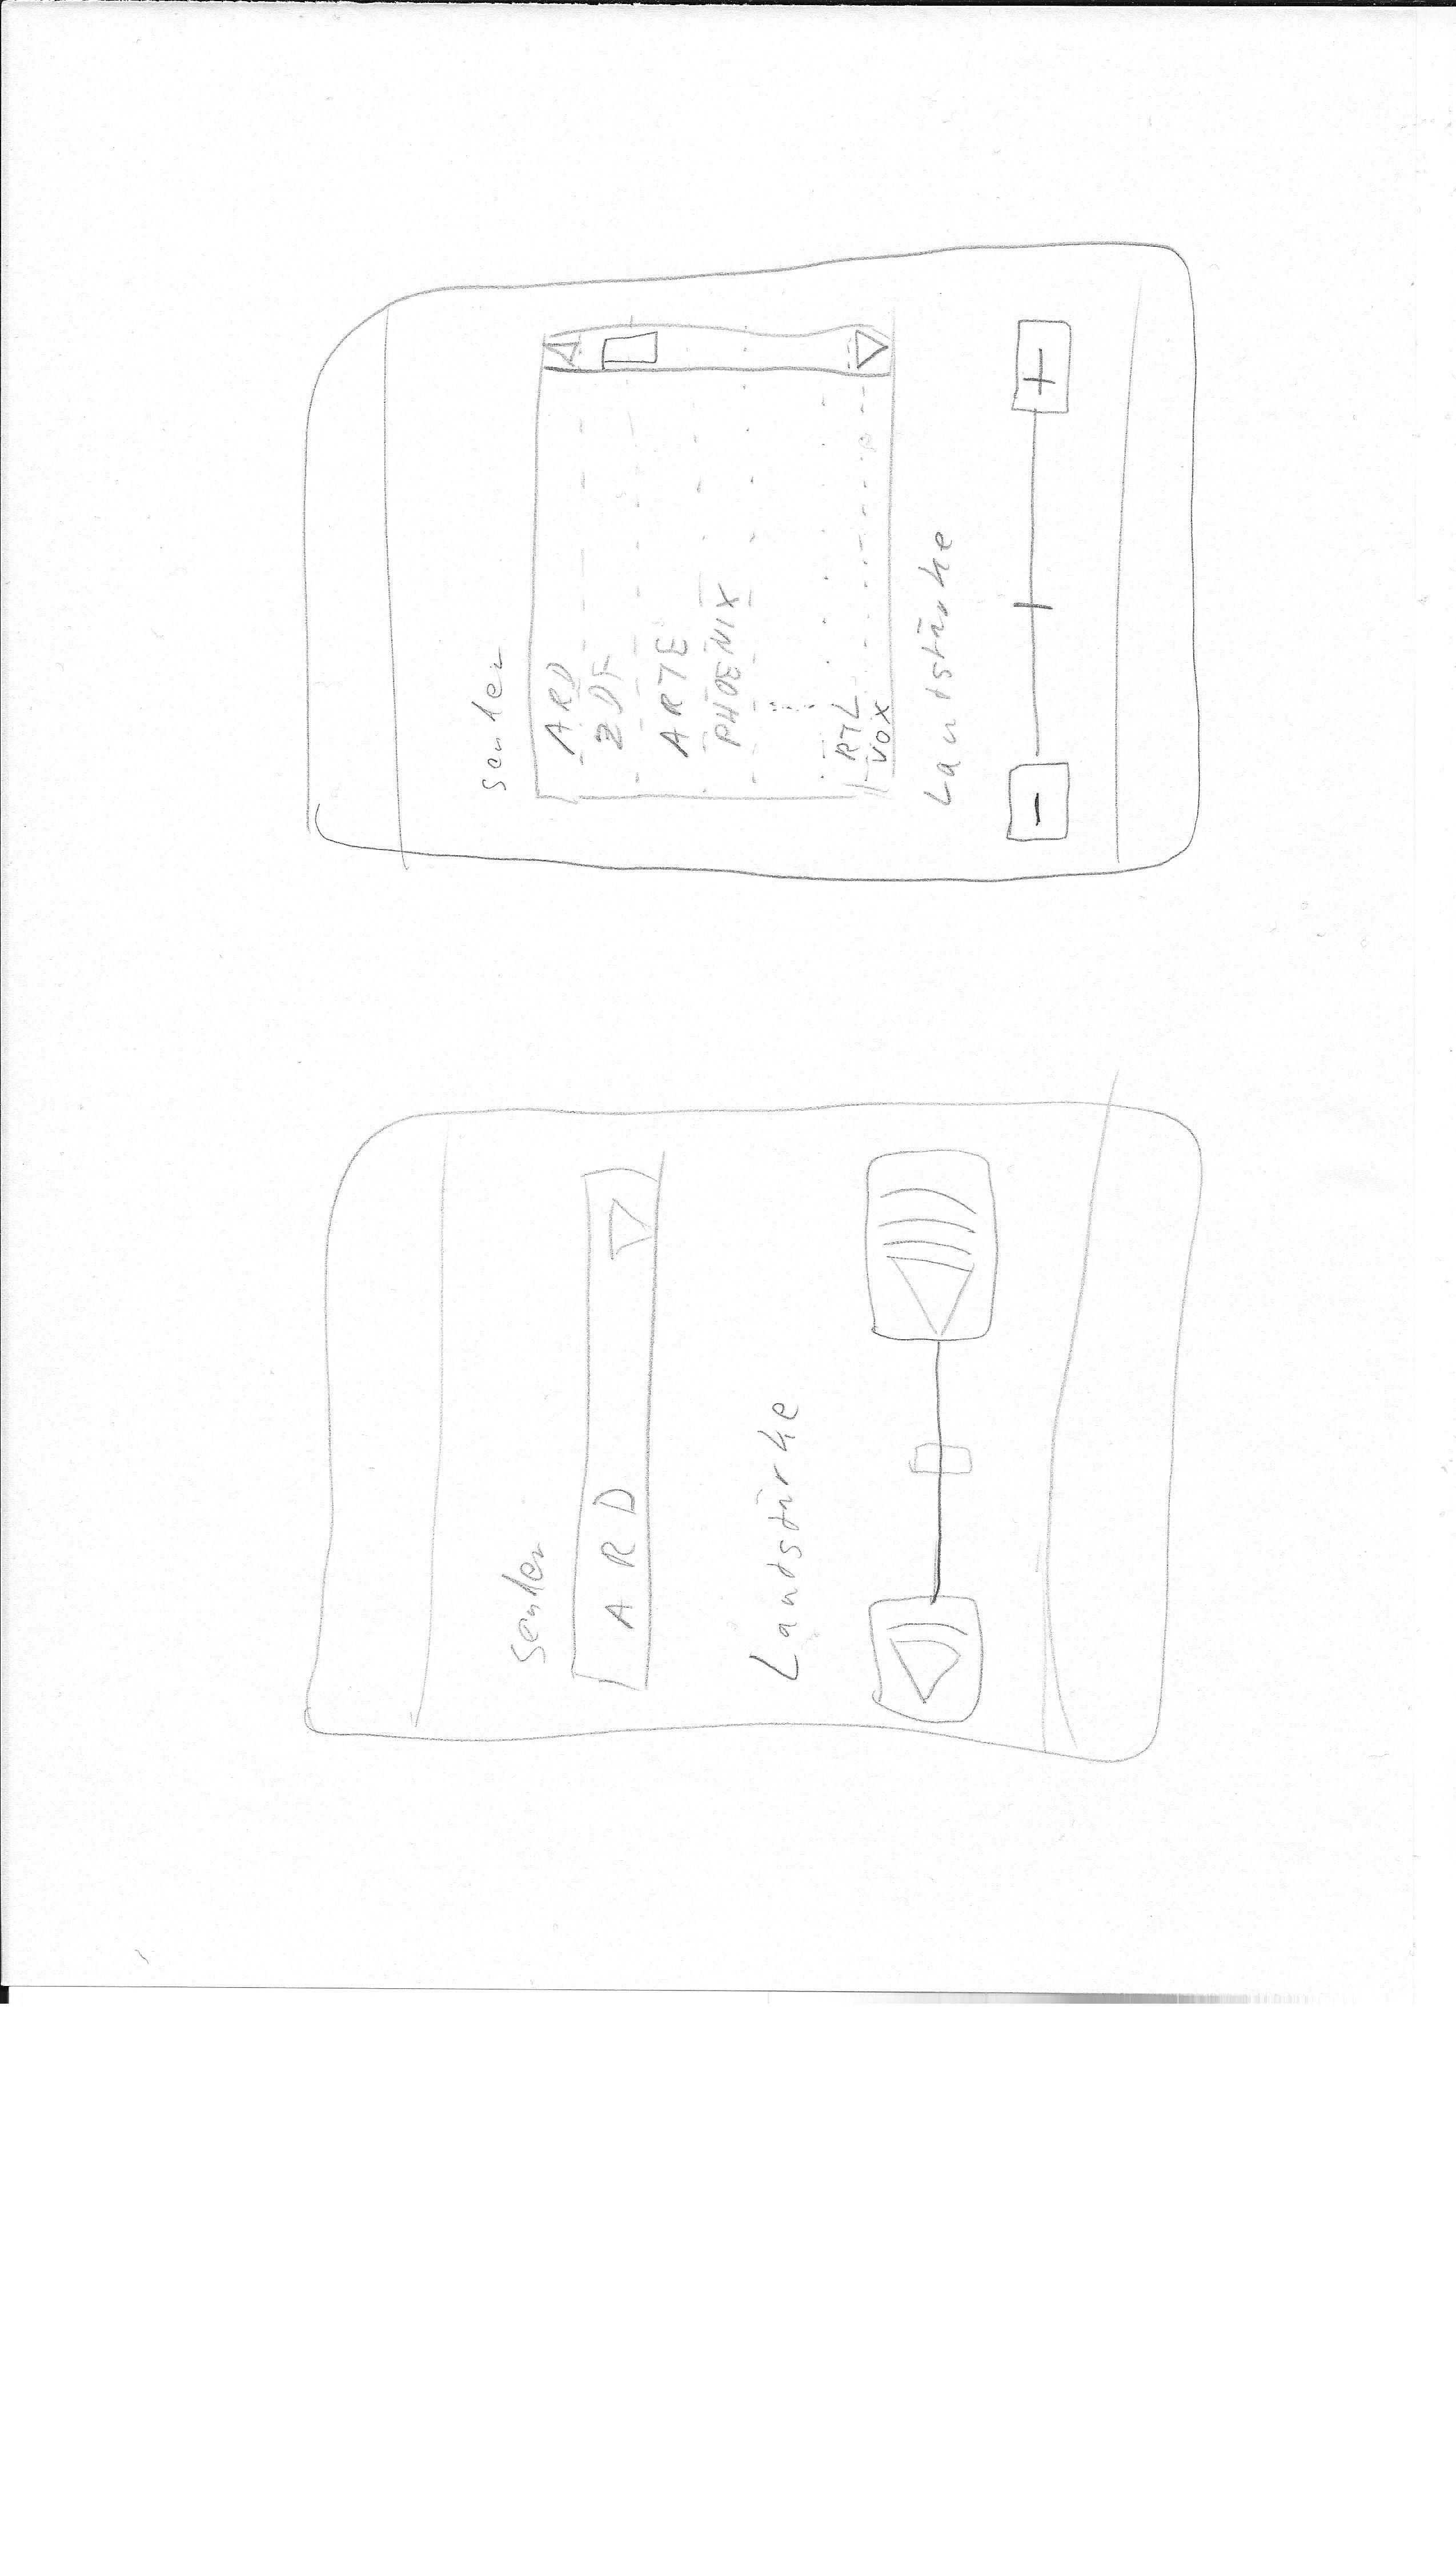
\includegraphics[scale=0.15]{sketch1}
		
		\item
		Den Schritt zur Entwicklung gleich mehrerer Papier-Prototypen mussten wir ebenso überspringen, da dies einen hohen Aufwand für vergleichbar geringen Nutzen verursacht hätte. Bei einer größeren App ist solch ein Schritt sicher sinnvoll, aber an der Funktionsfülle der App gemessen erschien uns dieser Schritt zu aufwendig. Wir sind stattdessen gleich dazu übergegangen einen Axure-Prototypen zu erstellen mit ebenso geringstmöglichem Aufwand.
		
		Daraus folgend haben wir uns mit dem optischen Aussehen nur am Rande beschäftigt und uns auf das funktionale Design konzentriert (Position und Bedienung der Elemente).
		
		Schließlich ergab sich daraus der folgende finale MockUp.
		
		\item Axure-Prototyp:\\
		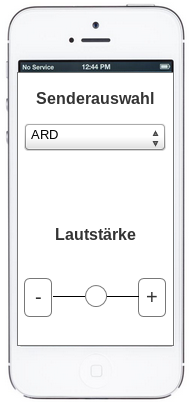
\includegraphics[scale=0.5]{AxurePrototyp}
		
	\end{enumerate}

\end{document}